\section{Mappery na inne formaty}
\paragraph{}Jak zostało wspomniane we wstępie, nasz mapper jest w stanie obsługiwać różne formaty, nie tylko .csv. Nie mniej jednak nie posiada on logiki do dokładnego mapowania z każdego z obsługiwanych formatów. Posiada on serię konwerterów między formatowych pozwalających tłumaczyć różne formaty na csv i na odwrót. Mechanizm działania samego mappera współpracuje tylko i wyłącznie z formatem csv, konwertery zapewniają dodatkową warstwę wsparcia poszerzając wachlarz wspieranych formatów. Konwersja ta, realizowana jest przy pomocy mechaniki \mintinline{php}|ExtensionProvider|, gdzie każdy konkretny "\textit{dostawca rozszerzeń}" funkcjonuje jako swojego rodzaju tłumacz między rdzeniem mappera a konkretnymi formatami.

\begin{figure}[ht]
	\centering
	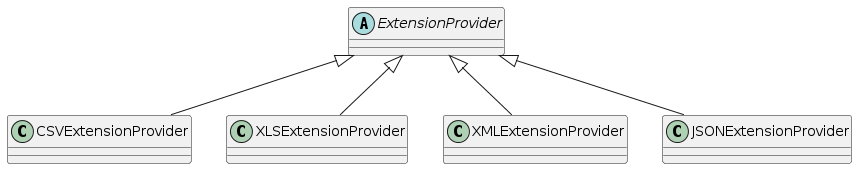
\includegraphics[width=1.0\textwidth]{materiały/hierarchia}
	\caption{Dostępni dostawcy formatów/rozszerzeń}
\end{figure}

Konkretnego dostawcę możemy wstrzyknąć do instancji mappera, przy pomocy metody \mintinline{php}|provideExtension(ExtensionProvider)|, nadpisując w ten sposób domyślnego dostawcę, tj. \mintinline{php}|CSVExtensionProvider|.

\begin{empty}
	\begin{minted}[
		startinline,
		linenos,
		frame=lines,
		framesep=2mm,
		baselinestretch=1.2,
		fontsize=\footnotesize,
		breaklines,
		obeytabs=true,
		tabsize=2,
		]{php}
public function main ()
{
	$this->csvMapper
	->provideExtension(new XMLExtensionProvider())
	->save($this->a);
	
	$x = $this->csvMapper
	->read("./A.csv", A::class);
}
	\end{minted}
	\vspace{-10pt}
	\captionof{listing}{Wstrzyknięcie dostawcy formatu XML}
\end{empty}

\paragraph{Uwaga:} Mimo, że jako ścieżkę podaliśmy plik z rozszerzeniem \textit{.csv}, to dostawca doklei do niego rozszerzenie \textit{.xml}.

\newpage
\subsection{CSVExtensionProvider}
Jest to domyślny oraz najprostszy dostawca, którego zadaniem jest tylko zapisać i odczytać podany plik. 

\begin{empty}
	\begin{minted}[
		startinline,
		linenos,
		frame=lines,
		framesep=2mm,
		baselinestretch=1.2,
		fontsize=\footnotesize,
		breaklines,
		obeytabs=true,
		tabsize=2,
		]{php}
namespace CSVMapper\ExtensionProvider;
use CSVMapper\ExtensionProvider\ExtensionProvider;

class CSVExtensionProvider implements ExtensionProvider
{
	public function write ($file, $csv)
	{
		file_put_contents($file, $csv);
	}
	
	public function read ($file)
	{
		return file_get_contents($file);
	}
}
	\end{minted}
	\vspace{-10pt}
	\captionof{listing}{CSVExtensionProvider}
\end{empty}

\subsection{XMLExtensionProvider}
Nieco bardziej zaawansowanym dostawcą jest, ten od formatu XML. Wykorzystując wbudowaną w język PHP bibliotekę \mintinline{php}|DOMDocument|, odpowiednio tworzy i parsuje pliki .xml na podstawie dostarczanych danych w formacie CSV.

\begin{empty}
	\begin{minted}[
		startinline,
		linenos,
		frame=lines,
		framesep=2mm,
		baselinestretch=1.2,
		fontsize=\footnotesize,
		breaklines,
		obeytabs=true,
		tabsize=2,
		]{xml}
<?xml version="1.0"?>
<Mapping>
	<Definition>
		<Field>moc</Field>
		<Field>id#</Field>
	</Definition>
	<Content>
		<Entity>
			<Value>245KM</Value>
			<Value> 66662740bf785</Value>
		</Entity>
	</Content>
</Mapping>
	\end{minted}
	\vspace{-10pt}
	\captionof{listing}{TestKompozycja-Silnik.csv.xml}
\end{empty}

\begin{empty}
	\begin{minted}[
		startinline,
		linenos,
		frame=lines,
		framesep=2mm,
		baselinestretch=1.2,
		fontsize=\footnotesize,
		breaklines,
		obeytabs=true,
		tabsize=2,
		]{xml}
<?xml version="1.0"?>
<Mapping>
	<Definition>
		<Field>model</Field>
		<Field> silnik@TestKompozycja\Silnik</Field>
		<Field>id#</Field>
	</Definition>
	<Content>
		<Entity>
			<Value>528i</Value>
			<Value> 66662740bf785</Value>
			<Value> 66662740bf77f</Value>
		</Entity>
	</Content>
</Mapping>
	\end{minted}
	\vspace{-10pt}
	\captionof{listing}{TestKompozycja-Samochod.csv.xml}
\end{empty}

\begin{empty}
	\begin{minted}[
		startinline,
		linenos,
		frame=lines,
		framesep=2mm,
		baselinestretch=1.2,
		fontsize=\footnotesize,
		breaklines,
		obeytabs=true,
		tabsize=2,
		]{php}
public function write ($file, $csv)
{
	$lines = explode("\n", $csv);
	$header = explode(";", array_shift($lines));
	
	$domDoc = new DOMDocument;
	$root = $domDoc->createElement('Mapping');
	...
	foreach ($header as $tok) {
		/**
		* Konwersja nagłowka ...
		*/
	}
	
	$content = $domDoc->createElement('Content');
	$root->appendChild($content);
	foreach ($lines as $line) {
		/**
		* Konwersja ciała ...
		*/
	}
	
	file_put_contents($file . ".xml", $domDoc->saveXML());
}
	\end{minted}
	\vspace{-10pt}
	\captionof{listing}{Fragment metody zapisu}
\end{empty}

\subsection{JSONExtensionProvider}
JSON jest jednym z najbardziej popularnych formatów, wymiany danych. Język PHP zawiera wbudowane funkcje do obsługi tego formatu, dlatego też, stworzenie konwertera nie stanowiło dużego wyzwania. 

\begin{empty}
	\begin{minted}[
		startinline,
		linenos,
		frame=lines,
		framesep=2mm,
		baselinestretch=1.2,
		fontsize=\footnotesize,
		breaklines,
		obeytabs=true,
		tabsize=2,
		]{php}
public function read ($file)
{
	$json = file_get_contents($file . ".json");
	$root = json_decode($json);
	
	$header = [];
	$entities = [];
	
	$first = (array) $root->entities[0];
	foreach ($first as $key => $value) {
		$header[] = $key;
	}
	
	foreach ($root->entities as $entity) {
		$values = [];
		foreach ((array) $entity as $value) {
			$values[] = $value;
		}
		$entities[] = implode(";", $values);
	}
	
	return implode(";", $header) . "\n" . implode("\n", $entities);
}
	\end{minted}
	\vspace{-10pt}
	\captionof{listing}{Metoda odczytu}
\end{empty}

\begin{empty}
	\begin{minted}[
		startinline,
		linenos,
		frame=lines,
		framesep=2mm,
		baselinestretch=1.2,
		fontsize=\footnotesize,
		breaklines,
		obeytabs=true,
		tabsize=2,
		]{json}
{
	"entities":[
		{
			"model":"528i",
			" silnik@TestKompozycja\\Silnik":" 666629a031291",
			" id#":" 666629a031289"
		}
	]
}
	\end{minted}
	\vspace{-10pt}
	\captionof{listing}{TestKompozycja-Samochod.csv.json}
\end{empty}

\begin{empty}
	\begin{minted}[
		startinline,
		linenos,
		frame=lines,
		framesep=2mm,
		baselinestretch=1.2,
		fontsize=\footnotesize,
		breaklines,
		obeytabs=true,
		tabsize=2,
		]{json}
{
	"entities":[
		{
			"moc":"245KM",
			" id#":" 666629a031291"
		}
	]
}
	\end{minted}
	\vspace{-10pt}
	\captionof{listing}{TestKompozycja-Silnik.csv.json}
\end{empty}

\begin{empty}
	\begin{minted}[
		startinline,
		linenos,
		frame=lines,
		framesep=2mm,
		baselinestretch=1.2,
		fontsize=\footnotesize,
		breaklines,
		obeytabs=true,
		tabsize=2,
		]{php}
		public function write ($file, $csv)
		{
			$lines = explode("\n", $csv);
			$header = explode(";", array_shift($lines));
			
			$root = (object) ["entities" => []];
			
			foreach ($lines as $line) {
				$toks = explode(";", $line);
				$newObj = [];
				for ($i = 0; $i < count($toks); $i++) {
					$newObj[$header[$i]] = $toks[$i];
				}
				$root->entities[] = (object) $newObj;
			}
			
			file_put_contents($file . ".json", json_encode($root));
		}
	\end{minted}
	\vspace{-10pt}
	\captionof{listing}{Metoda zapisu}
\end{empty}

\subsection{XLSExtensionProvider}
Ostatnim z obsługiwanych formatów jest XLS. W przypadku poprzednich formatów każdy rodzaj klasy był zapisany w osobnym pliku. W tym przypadku zostało zastosowane inne podejście - obiekty tych samych klas zapisywane są we wspólnych \textit{arkuszach}. Takie podejście wiąże się, z dodatkowymi komplikacjami. Format XLS posiada rygorystyczne ograniczenia dotyczące nazw arkuszy, dlatego też wszystkie nazwy musimy nadpisywać, tak aby spełniały one wspomniane kryteria. Dodatkowym problemem jest maksymalna długość nazwy, a mianowicie, jest to 31 znaków. Dlatego też został zastosowany manewr "numerowania" arkuszy. Ponieważ, osoba analizująca arkusz, własnoręcznie może mieć problemy z transkrypcją numerów na nazwy plików, do każdego zmapowanego pliku \textit{.xlsx}, dołączamy dodatkowy arkusz zawierający indeks nazw i odpowiadających im numerów. Ponadto język PHP natywnie nie wspiera formatu XLS, wymagana jest instalacja dodatkowej biblioteki \mintinline{php}|phpoffice/phpspreadsheet|. Aby tego dokonać, należy użyć narzędzia \textbf{composer} wywołując poniższe polecenie:\\
\mintinline{text}|# composer require phpoffice/phpspreadsheet|\\
Biblioteka ta, dodatkowo może wymagać konfiguracji ustawień samego PHP. Należy upewnić się, że poniższe moduły są włączone:\\
\mintinline{text}|extension=gd|\\
\mintinline{text}|extension=iconv|\\

\begin{figure}[ht]
	\centering
	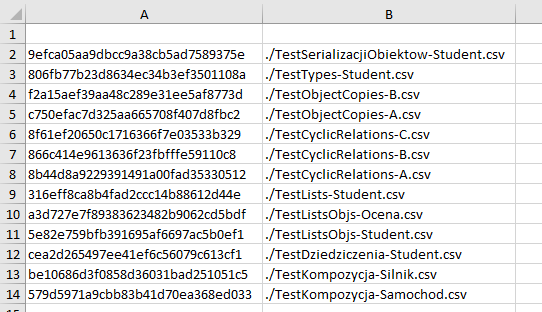
\includegraphics[width=0.9\textwidth]{materiały/excel1}
	\caption{Indeks nazw arkuszy}
\end{figure}

\begin{figure}[ht]
	\centering
	
\includegraphics[width=1.0\textwidth]{materiały/excel2}
	\caption{Widok dostępnych arkuszy w pliku}
\end{figure}

\begin{figure}[ht]
	\centering
	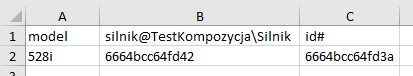
\includegraphics[width=0.7\textwidth]{materiały/excel3}
	\caption{Arkusz TestKompozycja-Samochod.csv}
\end{figure}